O TinyOS é o sistema operacional mais usado para auxiliar os programadores a desenvolverem aplicações para rede de
sensores sem fio de baixo consumo.
O modelo de programação provido é baseado em componentes e orientado a eventos.
Os componentes são pedaços de código reutilizáveis, onde são definidas claramente suas dependências e os serviços
oferecidos, por meio de interfaces. A linguagem \textit{nesc} implementa esse modelo estendendo a linguagem C.
É através da conexão (\textit{wiring}) de diversos componentes que o sistema é montado.

Já o modelo de programação orientado a eventos permite que o TinyOS rode uma aplicação, com somente uma linha de
execução, respondendo a diferentes interrupções de sistema, sem a necessidade de ações bloqueantes. 
Para isso todas as operações de entrada e saída são realizadas em duas fases.
Na primeira fase, o comando de E/S sinaliza para o hardware o que deve ser feito, e retorna imediatamente, dando continuidade a
execução. A conclusão da operação é sinalizada através de um evento, que será tratado pela segunda fase da operação de E/S.

O modelo de programação baseada em compontenes está intimamente ligada à programação orientada a eventos: Um componente
oferece a interface, implementando os comandos e sinalizando eventos relacionandos, enquanto outro componente
utiliza esta interface, através do uso dos comandos e da implementação dos tratadores de evento.

A divisão em componentes também facilita a implementação da camada de abstração de hardware. De forma que cada
plataforma tem um conjunto diferente de componentes para lidar com as instruções de cada hardware.
As abstrações providas são de serviços como sensoreamento, comunicação por rádio e armazenamento na memória flash.

\begin{figure}[htb]
\centering
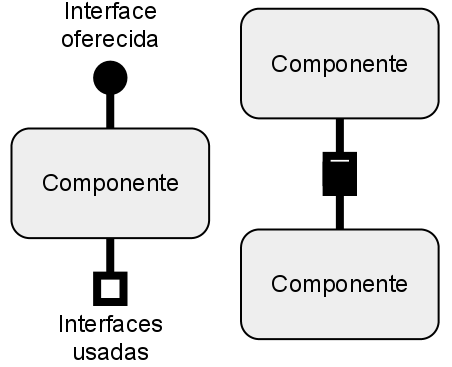
\includegraphics[scale=0.4]{images/interfaces-componentes.png}
\caption{Ilustração de componentes e suas interfaces}
\end{figure}

\paragraph{Exemplo}
A aplicação \textit{Blink}, no anexo~\ref{a:Blink}, é utilizada para ilustrar estes conceitos básicos. Esta aplicação
faz os LEDs da plataforma piscarem continuamente.
Toda aplicação utiliza uma configuração para descrever os componentes que serão usados, e quais são as conexões entre
as interfaces.
\lstinputlisting[caption=Configuração (BlinkAppC.nc), label=l:BlinkAppC]{srcs/BlinkAppC.nc}

Na listagem \ref{l:BlinkAppC}, pode-se ver que alguns dos componentes utilizados são \textit{MainC}, \textit{BlinkC}, \textit{LedsC}.
\textit{MainC} é o responsável pela inicialização do sistema. E indica o termino deste
processo através do evento \textit{booted}, da interface \textit{Boot} (mais detalhes na seção \ref{inicializacao}).
\textit{BlinkC} implementa a lógica da aplicação.
E \textit{LedsC} implementa as operações necessárias para acender ou apagar os Leds da plataforma.

O outro componente utilizado é um temporizador. O comando \textit{new} é usado para
criar instâncias de componentes genéricos. Isso permite a criação de cópias distintas de uma mesma funcionalidade.
Neste caso são criados três temporizadores diferentes.
Alguns componentes não podem ter cópias distintas, como o \textit{LedsC} que representa uma estrutra física do
sensor, logo não pode ser multiplicada.

Na listagem \ref{l:BlinkAppC} também são definidas as conexões das interfaces de cada componente.
A construção da linha 14, por exemplo, indica que o módulo \textit{BlinkC} utiliza a interface
oferecida por \textit{LedsC} para apagar ou acender os LEDs. 

A lógica da aplicação está implementada no componente \textit{BlinkC}, através da contrução de um módulo..
\lstinputlisting[caption=Interfaces usadas pelo módulo (BlinkC.nc), label=l:BlinkC1, lastline=10]{srcs/BlinkC.nc}
Na listagem \ref{l:BlinkC1}, estão especificadas as interfaces utilizadas, que formaram as conexões vistas na
configuração.

\lstinputlisting[caption={Eventos, Comandos, Postagem de tarefas (BlinkC.nc)} 
                ,label=l:BlinkC2, firstline=11, lastline=25, firstnumber=11]{srcs/BlinkC.nc}
Finalmente, na listagem \ref{l:BlinkC2}, é definida a lógica do componente principal da aplicação.
O tratador do evento \textit{Boot.booted} é o primeiro a ser ativado após a inicialização do sistema.
Dentro deste, é invocado o comando para inicializar os temporizadores. A periodicidade de cada um é definida pelo
parâmetro passado. E por último, é postada uma tarefa, cujos detalhes serão vistos a seguir.
O tratador do evento \textit{Timer0.fired}, toda vez que é ativado, invoca o comando responsável por acender/apagar o
LED 0. O mesmo acontece para os outros temporizadores.

\paragraph{Tasks}
O TinyOS também utiliza o conceito de procedimento postergados, chamados de tarefas (\textit{tasks}). As próprias
tarefas, comando e tratadores de eventos podem postar uma nova tarefas, a qual é enfileirada para execução posterior.
Esta será atendida, de forma síncrona, pelo escalonador.
Ser executada de forma síncrona, significa que tarefas não são preemptiva entre si. Portanto, se diversas tarefas
compartilha uma mesma variável, não haverá condições de corrida. Mais detalhes serão vistos na seção
\ref{modeloconcorrencia}.

\lstinputlisting[caption=Implementação de tarefas (BlinkC.nc), label=l:BlinkC3, firstline=37, lastline=41, firstnumber=37]{srcs/BlinkC.nc}

Na listagem \ref{l:BlinkC2}, existe um exemplo de uma postagem de tarefa. E na listagem \ref{l:BlinkC3}, um exemplo da
implementação de uma tarefa, que neste caso somente emite uma mensagem de depuração.

\paragraph{Interfaces}
Ao desenvolver aplicações mais complexas, é preciso desenvolver componentes intermediários. Estes devem além de usar,
também devem oferecer interfaces. Para oferecer novas interfaces, o programador deve declará-las, implementar seus 
comandos, e sinalizar seus eventos. O componente que usar estas interfaces, será responsável por utilizar os comandos e
implementar os tratadores de eventos.
\begin{lstlisting}[caption=interface, label=interface]
interface Send {
    command error_t send(message_t* msg, uint8_t len);
    command error_t cancel(message_t* msg);
    event void sendDone(message_t* msg, error_t error);
    command uint8_t maxPayloadLength();
    command void* getPayload(message_t* msg, uint8_t len);
}

module SendExample {
    provides interface Send;
}
implementation {
    command error_t Send.send(message_t* msg, uint8_t len) {
        //Implementacao do comando send.
        ...

        signal Send.sendDone(msg_var, SUCCESS);
    }
    ...
}
\end{lstlisting}
